%%%%%%%%%%%%%%%%%%%%%%%%%%%%%%%%%%%%%%%%%%%%%%%%%%%%%%%%%%%%%%%%%%%%%%%%%%%%%%%
%
% OCR - State of the art, possibilities and drawbacks
% 
%%%%%%%%%%%%%%%%%%%%%%%%%%%%%%%%%%%%%%%%%%%%%%%%%%%%%%%%%%%%%%%%%%%%%%%%%%%%%%%
\chapter{OCR - State of the art, possibilities, and drawbacks}
\label{cha3}

During the processing of a form, the image of it is not only scanned. To enhance the retrieved information and thus optimize our result we additionally make use of OCR.

The process of retrieving data, for instance in form of characters or numbers, requires several steps. These steps are also shown in figure \ref{ocrSteps}. In the beginning, the image to be processed is converted to a gray-scale image. Then preprocessing takes place. In the processing phase, several algorithms such as noise-reduction and the canny-edge-algorithm are applied on the image to reduce irritating and / or unnecessary information in the image and to enhance contrast.

\begin{figure}[htbp!]
\centering
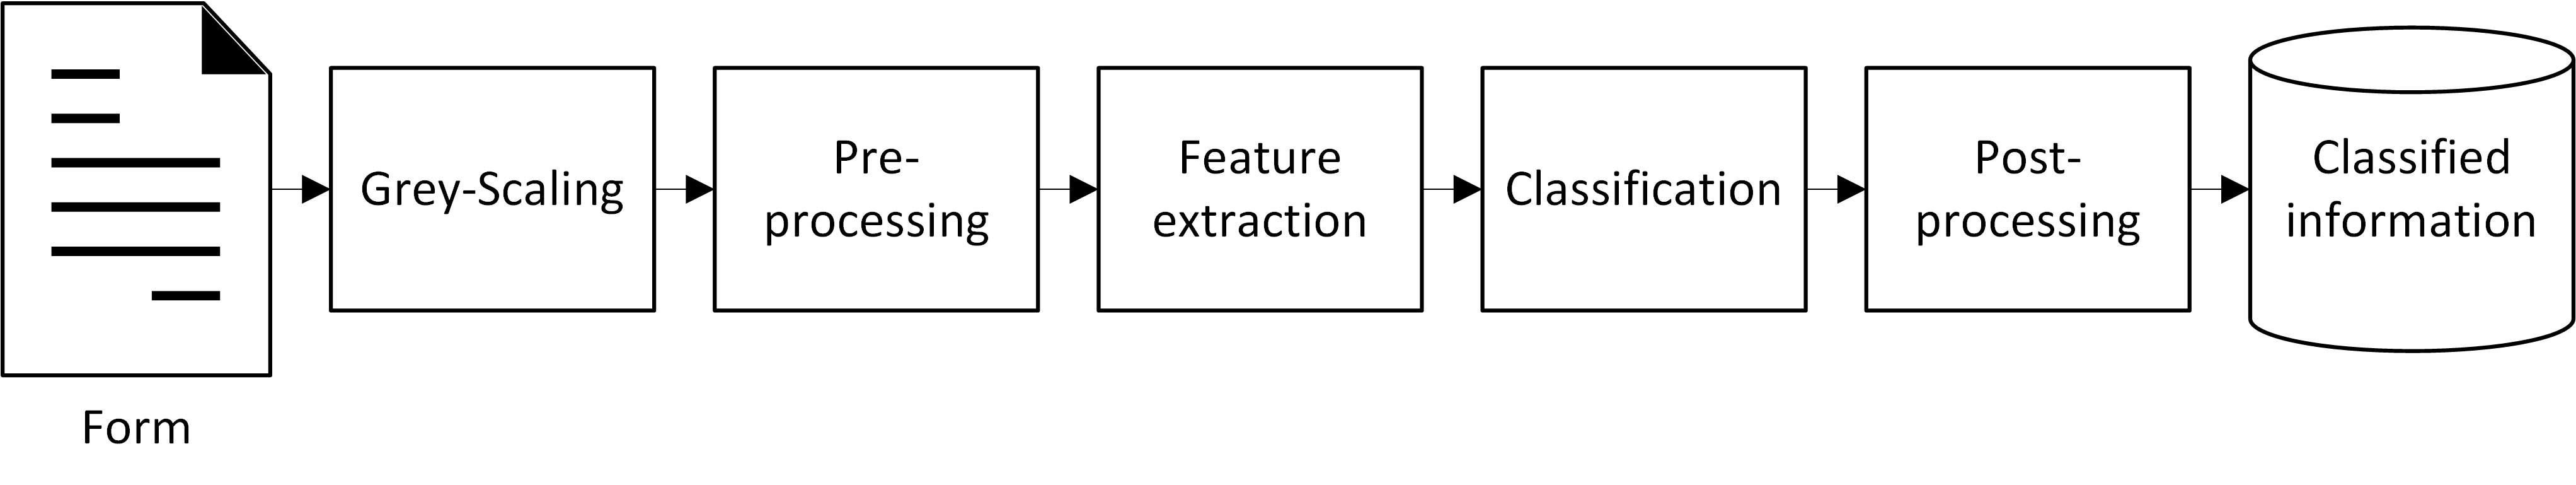
\includegraphics[scale=0.9]{Images/OCR/Steps_Of_OCR.png}
\caption{Steps of OCR \label{ocrSteps}}
\end{figure}

After that, features are extracted. Those features are single characters whose vectors are defined afterwards. With the information about the feature vector, it is possible to classify each character (and to detect which character of the alphabet is most likely to be represented by the feature).

When all characters have been classified, post-processing takes place. Here, possible failures can be corrected, for example by comparing words with a predefined dictionary.

The whole process of OCR is part of research since decades and several papers, dissertations, and books have been published on the matter\cite{impedovo91}\cite{Mori99}\cite{Wang15}. Developing our own OCR algorithm would not only exceed the size of this master thesis but also most likely retrieve less successful results than already developed and improved algorithms. Instead, this chapter will introduce several available OCR algorithms and compare open source solutions to find the best fit for our need.

\section{Currently available OCR algorithms}
\label{sec3.1}

OCR has been of interest for companies over many years. Hence we expect several possible solutions we could choose. As the amount of solutions can easily be very high we want to reduce the presented solutions to a maximum amount of 10.

Each description of a solution will contain information about the license used, the supported operating systems, programming languages used as well as if there is a software development kit. Also, general information about the company will be given, the currently released version of the solution and the release date and, if existent, the number of languages supported.

\subsection{ABBYY Fine Reader}
\label{sec3.1.1}

ABBYY Fine Reader is a proprietary solution from the identically named company ABBYY founded in 1989. It is usable for all three operating systems, whereby Linux-distributions are only supported as a command-line-interface. ABBYY supports a SDK for all three operating systems. Although it is written in C/C++ there exists a wrapper for Java development for Linux and Windows\cite{abbyy16}. 

The SDK is currently in Version 11, it supports 185 languages, the latest update was on 03.10.2016.

\subsection{Anyline SDK}
\label{sec3.1.2}

Anyline is an Austrian company founded in 2013 which aims at OCR solutions for mobile systems. They offer their SDK as a free license for non-commercial use. However, as they are focused on mobile systems, they do not explicitly support Windows-Desktop, Linux or MacOS.

It can be developed with Java and Objective-C as well as Swift, C\#, and Javascript. The current version of the SDK is 3.8.1 and has been released on 13.01.2017.

Currently supported are two languages: English and German.

\subsection{Asprise OCR}
\label{sec3.1.3}
Asprise has been founded in 1998 in Singapore. The company offers OCR SDKs in various programming languages (Java, C\#, VB.NET, Python, C/C++, and Delphi Pascal). The SDKs are under loyalty-free license and therefore proprietary. More than 20 languages are supported, English and German are included.
The SDK supports Windows, MacOS, and Linux, whereby support of multiple operating systems at once increases the price.

\subsection{GOCR}
\label{sec3.1.4}
GOCR is an OCR application started by Joerg Schulenburg in 2000. The program is developed under the GNU Public License.\footnote{The project can be found here: \url{http://jocr.sourceforge.net/}, last visited on 06.03.2016}

The latest version is 0.5 and has been released in March 2013. It is working under Windows, Linux and MacOS. The code is written in C, but it is not known if there is a SDK which enables usage of the application inside another application. The number of supported languages is not stated on the project page.

\subsection{LEADTOOLS}
\label{sec3.1.5}
Leadtools is an American company founded in 1990 and offers various products in the range of document and image processing. 

The Leadtools OCR Engine can be used as an SDK and integrated into another application. Development with the SDK is possible with C\# and VB as well as C/C++ and Java (and some others). The engine supports more than 40 languages, containing German and can be used on Windows, Linux and MacOS. 

The current version of the SDK is 19 and has been released in December 2014.

\subsection{MathOCR}
\label{sec3.1.6}
MathOCR is a document recognition system written in Java with focus on formulas. The MathOCR project started in March 2014 and is based on the GNU General Public License.\footnote{The source code can be found here: \url{https://sourceforge.net/projects/mathocr/}, last visited on 06.03.2017}

The current version of the application is 0.0.3, which was released in May 2015 and is therefore still in a pre-alpha status. It can be used on Windows, Linux, and MacOS. A number of supported languages is not stated on the project page.

\subsection{OCROpus}
\label{sec3.1.7}
The OCRopus Open Source OCR System is an open source system developed and maintained by the German Research Laboratory for Artificial Intelligence under guidance by Thomas M. Breuel\footnote{The source code can be found here: https://github.com/tmbdev/ocropy, last visited on 06.03.2017}. It is licensed under the Apache 2.0 License. It was first published in 2008 \cite{Breuel08}.

The command-line application is written in Python and C++ and only supports Linux as Operating System. It currently uses the Tesseract engine (as explained in \ref{Tesseract}) as a text line recognizer but will replace it in the future. 

The current stable version is 1.0 and has been released in November 2014. The number of supported languages is unknown, whereby it is able to work with latin-based languages.

\label{OCRad}
\subsection{OCRad}
OCRad is a free OCR application under the GNU Public License and part of the GNU project \footnote{The project can be found here: \url{https://www.gnu.org/software/ocrad/}, last visited on 06.03.2017}. Antonio Diaz Diaz developed the application since 2003.

The current version is 0.25 and has been released in April 2015. It comes as a stand-alone console application but can also be used in the background by other applications.

\label{OmniPage}
\subsection{OmniPage Capture SDK}
The Nuance Communication Inc. offers an OCR tool called OmniPage Capture SDK, which enables document processing on Windows, Linux, and MacOS. Depending on the underlying operating system it supports C/C++, Objective-C or C\# and VB.NET.

The current version is 20 and has been released in 2016. It supports over 120 languages (German included).

\label{Tesseract}
\subsection{Tesseract}
The Tesseract OCR Engine historically was an early project developed by Hewlett Packard between 1984 and 1994. In 2005, it was put on an open source license. It is currently maintained by Google under the Apache 2.0 license \cite{smith07}.

Tesseract is originally written in C/C++ and can be used on Windows, MacOS and Linux\footnote{The source code for tesseract can be found here: https://github.com/tesseract-ocr, last visited on 06.03.2017}. There also exists a wrapper which allows development in Java, the open source project Tess4J\footnote{The wrapper can be found on: \url{http://tess4j.sourceforge.net/}, last visited on 06.03.2017}.

The current stable version of the Tesseract is 3.04.01 and has been released in February 2016. It supports over 100 languages (including German). 

\section{Comparison between open source algorithms}
\label{sec3.2}
While several companies exist that offer good OCR libraries and SDKs, we will stick to free software in order to increase the acceptance for SMEs. In a later state of the application, it could be possible to switch to a proprietary solution in order to increase our OCR efficiency. Until then, we will decide for the best fitting open source algorithm library. We implemented a preprocessing routine on top of the OCR application's software stack to enable automation as much as possible. This is explained in \ref{sec5.4}.

Upon the 10 presented solutions, only 5 are free for use. These are: GOCR, Tesseract, OCROpus, MathOCR, and OCRad.

The following table shows the named solutions and shows their differences regarding their version, the latest release date, the supported programming languages and operating systems as well as the license they are put on:

\begin{table}[!htb]
\centering
\resizebox{\textwidth}{!}{%
\begin{tabular}{lccccc}
\hline
Application                                                               & \textbf{GOCR}                                                                           & \textbf{Tesseract}                                                                           & \textbf{OCROpus}                                                               & \textbf{MathOCR}                                                                        & \textbf{OCRad}                                                                          \\ \hline
Version                                                                   &0.5                                                             & 3.04.01                                                              & 1.0                                                    & 0.0.3                                                           & 0.25                                                            \\ \hline
Release Date                                                              & 03.2013                                                         & 02.2016                                                              & 11.2014                                                & 05.2015                                                         & 04.2015                                                         \\ \hline
\begin{tabular}[c]{@{}l@{}}Supported Programming\\ Languages\end{tabular} & C                                                               & \begin{tabular}[c]{@{}c@{}}C/C++, \\ Java (with Tess4J)\end{tabular} & \begin{tabular}[c]{@{}c@{}}C++, \\ Python\end{tabular} & Java                                                            & C++                                                             \\ \hline
\begin{tabular}[c]{@{}l@{}}Supported Operating\\ Systems\end{tabular}     & \begin{tabular}[c]{@{}c@{}}Windows, Linux,\\ MacOS\end{tabular} & \begin{tabular}[c]{@{}c@{}}Windows, Linux,\\ MacOS\end{tabular}      & Linux                                                  & \begin{tabular}[c]{@{}c@{}}Windows, Linux,\\ MacOS\end{tabular} & \begin{tabular}[c]{@{}c@{}}Windows, Linux,\\ MacOS\end{tabular} \\ \hline
License                                                                   & \begin{tabular}[c]{@{}c@{}}GNU Public \\ License\end{tabular}   & Apache 2.0                                                           & Apache 2.0                                             & \begin{tabular}[c]{@{}c@{}}GNU Public \\ License\end{tabular}   & \begin{tabular}[c]{@{}c@{}}GNU Public \\ License\end{tabular}   \\ \hline
\end{tabular}%
}
\caption{Comparison between different OCR engines}
\label{ocrEngineComparison}
\end{table}

MathOCR is a relatively young application and therefore in a pre-alpha state. OCRad and GOCR are one step closer to the first major release. OCROpus has reached that state on November 2014. Tesseract is already on Version 3.04 and has recently released an alpha version of 4.0.

While Tesseract, OCROpus, and OCRad are supporting C++, GOCR is only working with C whereas MathOCR is only Java. Tesseract is supporting C and Java as well (while using Tess4J as a wrapper). OCROpus instead is working with Python, too.

All solutions support Windows, Linux, and MacOS except OCROpus, which is only working on Linux.

While GOCR, MathOCR, and OCRad are licensed under the GNU Public License, Tesseract and OCROpus are licensed under the Apache 2.0 License. The difference between those two is mainly the following: Applications that are developed with the usage of another program under the GNU Public License have to be licensed under the GNU Public License as well. The Apache 2.0 license allows usage of other application and enables free choice of licensing, but requires the mentioning of the underlying use of an Apache 2.0 licensed application.

\label{OCRDecision}
\section{Decision finding and explanation}
In the beginning of this thesis, it was defined that the application should work on a Linux based operating system and be written in Java. While all presented solutions support Linux as an Operating System, not all of them work with Java as a programming language. In addition to that, OCROpus only supports Linux, which is fine for the current focus of the application but could be an issue later on, if it should be ported to another operating system.

MathOCR is in a pre-alpha state which makes it difficult to use due to several missing functionalities and persistent bugs in the code. As it is mostly focused on mathematical equations and formulas, we will not consider MathOCR any longer, even though it supports Java as a programming language. 

As explained in section \ref{sec3.2}, the GNU Public License requires our application to be licensed under the GNU Public License as well if we use another code which is licensed under this license. Therefore, the Apache 2.0 license is considered better, as it allows us to decide about the license for ourselves.

In the interest of the application, we want to use solutions that are up-to-date and are still under development. Therefore, the latest release date gives us insights about the activity on a project. Since a lot of open source projects suffer from missing developers, we expect longer development cycles. But the last version of GOCR has been released around 4 years ago. Hence we consider GOCR as not up-to-date anymore.

The following table shows the solutions again, but with underlying colors regarding their ability to fit to our problem. Green is used as the best fit, whereas red significates a major problem. Yellow shows that this attribute is not as good as others but no kick-out criterion. 

\begin{table}[!htb]
\centering
\resizebox{\textwidth}{!}{%
\begin{tabular}{lccccc}
\hline
Application                                                               & \textbf{GOCR}                                                                           & \textbf{Tesseract}                                                                           & \textbf{OCROpus}                                                               & \textbf{MathOCR}                                                                        & \textbf{OCRad}                                                                          \\ \hline
Version                                                                   & \cellcolor[HTML]{FFFE65}0.5                                                             & \cellcolor[HTML]{96D532}3.04.01                                                              & \cellcolor[HTML]{96D532}1.0                                                    & \cellcolor[HTML]{FD4703}0.0.3                                                           & \cellcolor[HTML]{FFFE65}0.25                                                            \\ \hline
Release Date                                                              & \cellcolor[HTML]{FD4703}03.2013                                                         & \cellcolor[HTML]{96D532}02.2016                                                              & \cellcolor[HTML]{FFFE65}11.2014                                                & \cellcolor[HTML]{96D532}05.2015                                                         & \cellcolor[HTML]{96D532}04.2015                                                         \\ \hline
\begin{tabular}[c]{@{}l@{}}Supported Programming\\ Languages\end{tabular} & \cellcolor[HTML]{FD4703}C                                                               & \cellcolor[HTML]{96D532}\begin{tabular}[c]{@{}c@{}}C/C++, \\ Java (with Tess4J)\end{tabular} & \cellcolor[HTML]{FD4703}\begin{tabular}[c]{@{}c@{}}C++, \\ Python\end{tabular} & \cellcolor[HTML]{96D532}Java                                                            & \cellcolor[HTML]{FD4703}C++                                                             \\ \hline
\begin{tabular}[c]{@{}l@{}}Supported Operating\\ Systems\end{tabular}     & \cellcolor[HTML]{96D532}\begin{tabular}[c]{@{}c@{}}Windows, Linux,\\ MacOS\end{tabular} & \cellcolor[HTML]{96D532}\begin{tabular}[c]{@{}c@{}}Windows, Linux,\\ MacOS\end{tabular}      & \cellcolor[HTML]{FFFE65}Linux                                                  & \cellcolor[HTML]{96D532}\begin{tabular}[c]{@{}c@{}}Windows, Linux,\\ MacOS\end{tabular} & \cellcolor[HTML]{96D532}\begin{tabular}[c]{@{}c@{}}Windows, Linux,\\ MacOS\end{tabular} \\ \hline
License                                                                   & \cellcolor[HTML]{FFFE65}\begin{tabular}[c]{@{}c@{}}GNU Public \\ License\end{tabular}   & \cellcolor[HTML]{96D532}Apache 2.0                                                           & \cellcolor[HTML]{96D532}Apache 2.0                                             & \cellcolor[HTML]{FFFE65}\begin{tabular}[c]{@{}c@{}}GNU Public \\ License\end{tabular}   & \cellcolor[HTML]{FFFE65}\begin{tabular}[c]{@{}c@{}}GNU Public \\ License\end{tabular}   \\ \hline
\end{tabular}%
}
\caption{Advantages and disadvantages of different OCR engines}
\label{ocrEngineRating}
\end{table}

As shown in the table, MathOCR will not fit our needs as it is a pre-alpha version. GOCR is outdated and also supports only C as a programming language. OCROpus and OCRad only support C++ (and in the case of OCROpus Python). In addition to that, OCROpus could be a problem when porting the application to other operating systems whereas OCRad is licensed under the GNU Public License. 

Hence the Tesseract seems to be the best fit for our application. It is consistently updated and improved. Considering the development history, the application itself has grown mature. The possibility to work with Tess4J enables the usage of it with Java. Multiple operating systems are supported and the Apache 2.0 license enables us to decide for ourselves under which license we will put the application.